\documentclass{article}
\usepackage{assumptionsofphysics}
\usepackage{graphicx}
\graphicspath{{images/}}
\begin{document}


\title{Derivation Steps}

\section{Introduction}

	The purpose of this work is to re-derive Hamiltonian and Lagrangian mechanics. Historically the basis for the laws of physics were generalized experiences. These laws were rooted in the physical world rather than a mathematical one. As they are treated now, Hamiltonian and Lagrangian mechanics lack this physicality. They are taught as mathematical reformulations of Newtonian Mechanics which they are not. This work will begin with basic physical assumptions about a system in order to show it obeys Hamiltonian and Lagrangian Mechanics with a more physical justification. We will start with physical assumptions, then translate those assumptions into precise mathematical definitions. This will lead us to our results. \emph{expand justification and explanation of methods and rationale.}
	
Diagram 1 here

\section{Infinitesimal Reducibility}
	
\begin{assump}[Infinitesimal reducibility]
	The state of the system is reducible to the state of its infinitesimal parts. That is, giving the state of the whole system is equivalent to giving the state of its parts, which in turn is equivalent to giving the state of its subparts and so on. This relationship holds the the other way as well. Giving the states of the smallest subdivisions of the system is equivalent to giving the state of the whole system.
\end{assump}
	
	\emph{Explain in practical terms what reducibility is}
	
	What does it mean physically for a system to be reducible? Let's consider a ball of reducible material that we throw through the air. This ball will follow some path. We can fully describe the state of the ball by its motion through the air. Now, say we draw a red dot on this ball. Then if we fully describe the motion of the ball, we have also described the motion of the red dot. The ball is a reducible system thus giving the state of the whole is equivalent to giving the state of the parts. The internal dynamics of the system are accessible meaning we can know the states of the parts of the system given knowledge of the state of the whole. Additionally if we give the motion of the red dot through the air, as well as how the rest of the ball moves, we know the motion of the whole ball. The state of the whole system can be known from the states of its parts. 
	
\begin{figure}[!ht]
\centerline{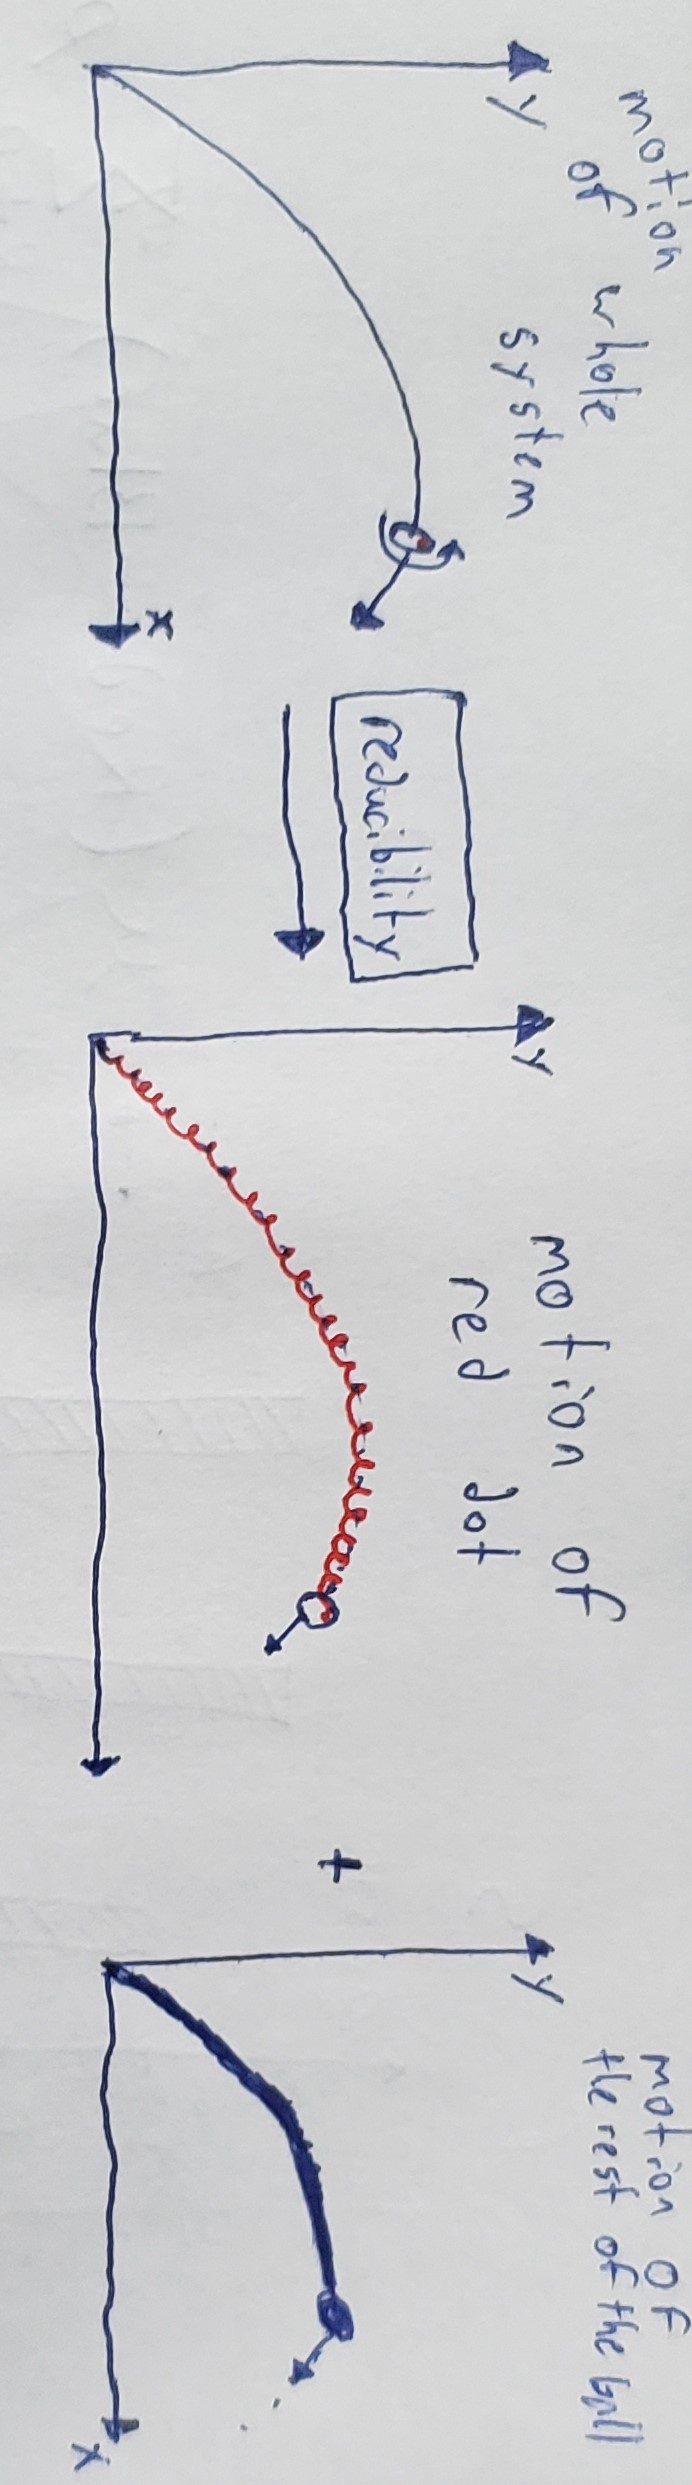
\includegraphics[width=\linewidth,angle=90,scale=.25]{reddotdiagram.jpg}}
\caption{Motion of our ball and red dot example. Because this system is reducible we can break the whole system into its parts.}
\end{figure}

	\emph{motivate the uniqueness of the distribution}	
	
	Each state of the whole system is uniquely determined by the states of its parts, meaning that given the set of states of the parts, we can determine exactly the state of the whole system. Two identical systems are in the same state if and only if all of their parts are in the same states. The same is true the other way around. The states of the parts of the system are uniquely determined by the state of the whole. Thus we have an invertible map between the state of our whole system and the states of its parts. In our example, this means that there is exactly one path traveled by the red dot per distinct state of the whole ball. So if we throw the ball with no angular velocity, the red dot will travel a parabola through the air. We could then throw the ball with the same linear velocity so that its center of mass travels the same path as before, but if the ball is spinning we have a different path traveled by the red dot. So from two distinct states of the overall system, one with angular velocity one without, we find two distinct sets of states of the parts of the system. One spiraling trajectory and one parabola.
		
	 %If we consider a ball of irreducible material i.e. an electron, we cannot describe the state of a dot drawn on its surface. We could not say for instance that a photon scattering with that electron interacts specifically with the part of the electron with the dot. That is because the electron is not reducible; we cannot describe the state of the electron by breaking it into smaller parts and describing those parts. We cannot describe a process in which something interacts with only part of the electron. 
	 
	 \emph{Describe what the process of subdivision is, and define the particle as the limit of that process}
	 
	 We have described reducibility in general, but what does it mean to be infinitesimally reducible? If a system is infinitesimally reducible we can subdivide it as many times as we want and the smallest subdivisions will still be themselves reducible. If we imagine that we divide our system until we approach the limit of recursive subdivision we will arrive at a collection of infinitesimally small parts of the system; we call these smallest subdivisions classical particles. What does this mean physically? Continuing our previous example, imagine we cover the surface of the ball in red dots. We then remove these dots and replace each of them with a number of smaller dots. We repeat this process until the radius of the dots is approaching zero. Because the ball is a reducible system, given the state of the whole ball, we know the states of all of the red dots drawn on it. It is important to note that the dots do not ever become points. They are always have radii that are greater than zero. No dot is a point particle, rather they are infinitesimally small subdivisions. We can always divide them again. The limit of these subdivisions are our classical particles. Assuming a system to be infinitesimally reducible means that given the state of the whole system, we can describe the states of all the infinitesimally small parts of the system. Now we must codify this idea formally.
	 
	 \emph{translate 3 paragraphs above into formal system}
	
	Let's start with a discrete system as it is conceptually simpler. Consider a box with a fixed number of balls of varying colors as our whole system. Suppose the state of the whole system will be defined by the number of balls of each color. We can formally define the \textit{state space} of the balls as $\mathcal{S}$ which spans all possible colors. Each ball is at a point $s \in \mathcal{S}$ corresponding to its color. We call the state space of our whole system $\mathcal{C}$ which spans all possible color combinations of the balls. One state of the whole system is a point $c \in \mathcal{C}$. For a state $c \in \mathcal{C}$ we can define the number of balls of each color as a \textit{distribution}, $\rho$, over the state space $\mathcal{S}$ of the balls. This distribution is unique to each state of the whole system. Two identical systems are in the same state if and only if their distributions are equivalent. For each distinct state $c \in \mathcal{C}$ of the whole system, we have exactly one $\rho$. 

\begin{figure}[!ht]
\centerline{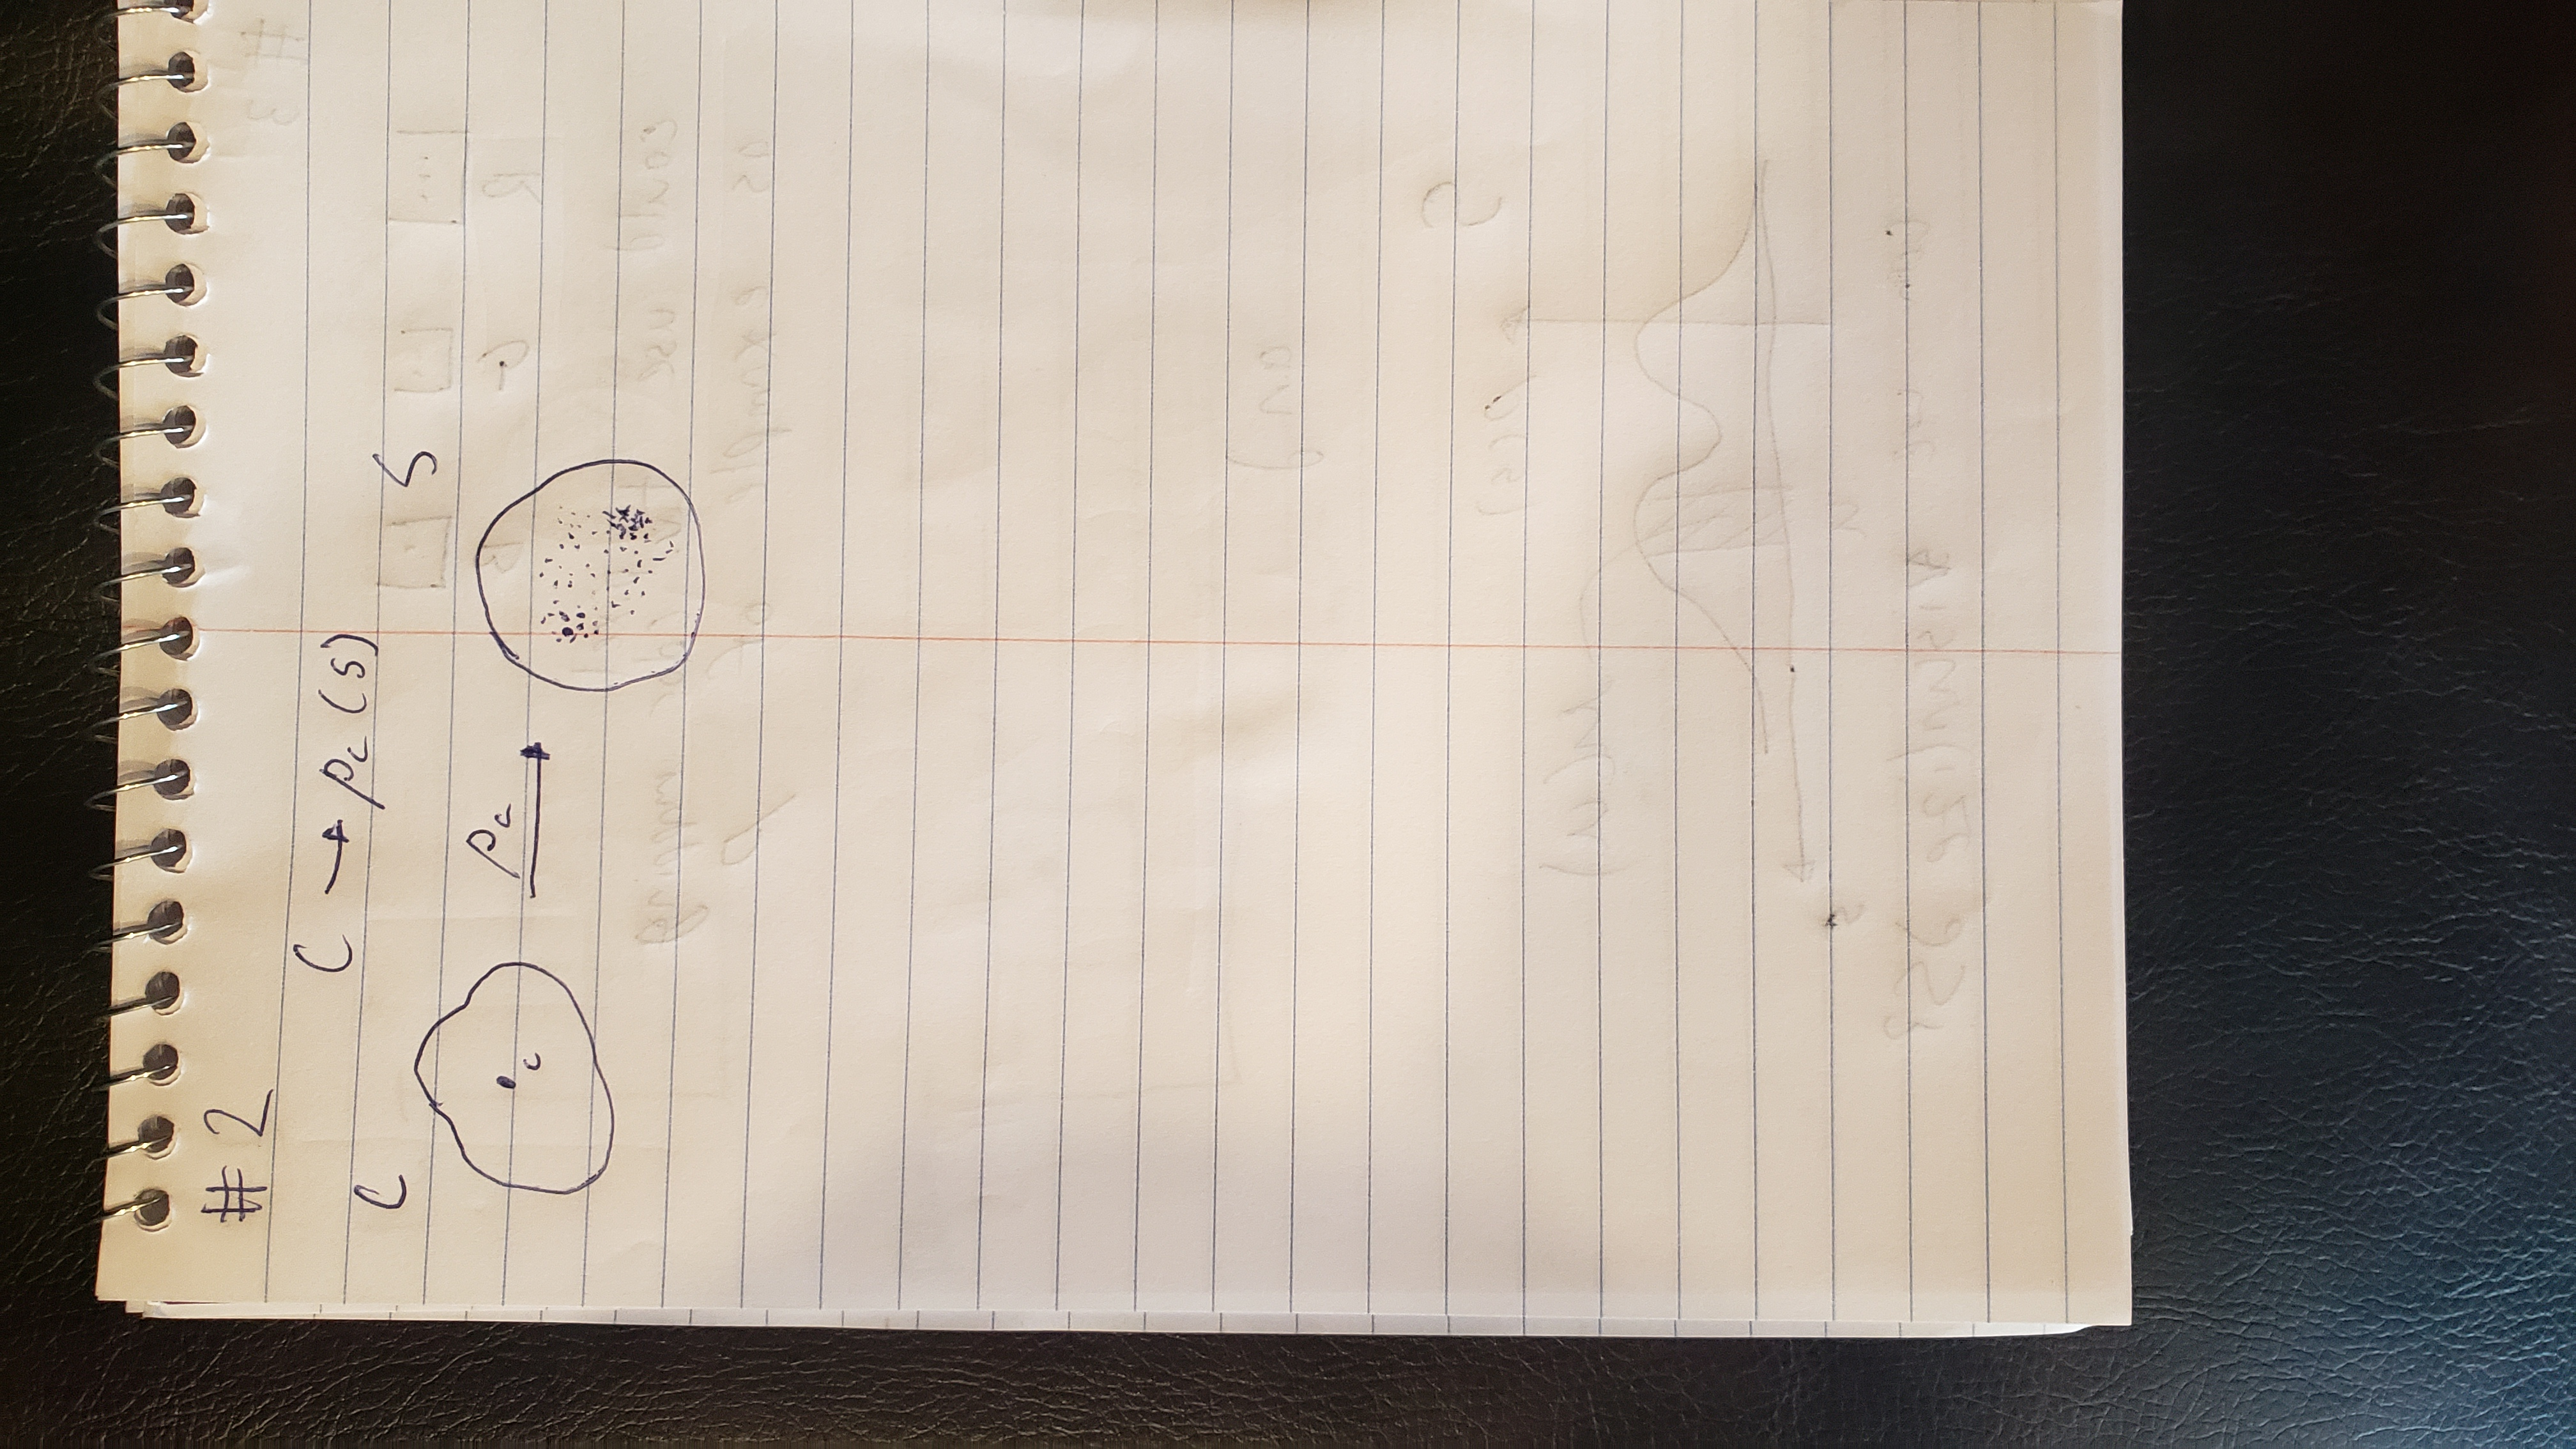
\includegraphics[width=\textwidth,angle=-90,scale=.35]{diagram2.jpg}}
\caption{Two different states of the system map to two different distributions of the parts of the system over $\mathcal{S}$.}
\end{figure}
	
	For each subset of colors in $\mathcal{S}$, we can count the number balls that are those colors; call this counting function $\mu : \mathcal{S} \to \mathbb{R}$. That is, for each $U \subset \mathcal{S}$ we have $\mu(U) = \sum_{s \in U} \rho(s)$. We will normalize this counting function by defining $\mu(S) = 1$.
	
\begin{figure}[!ht]
\centerline{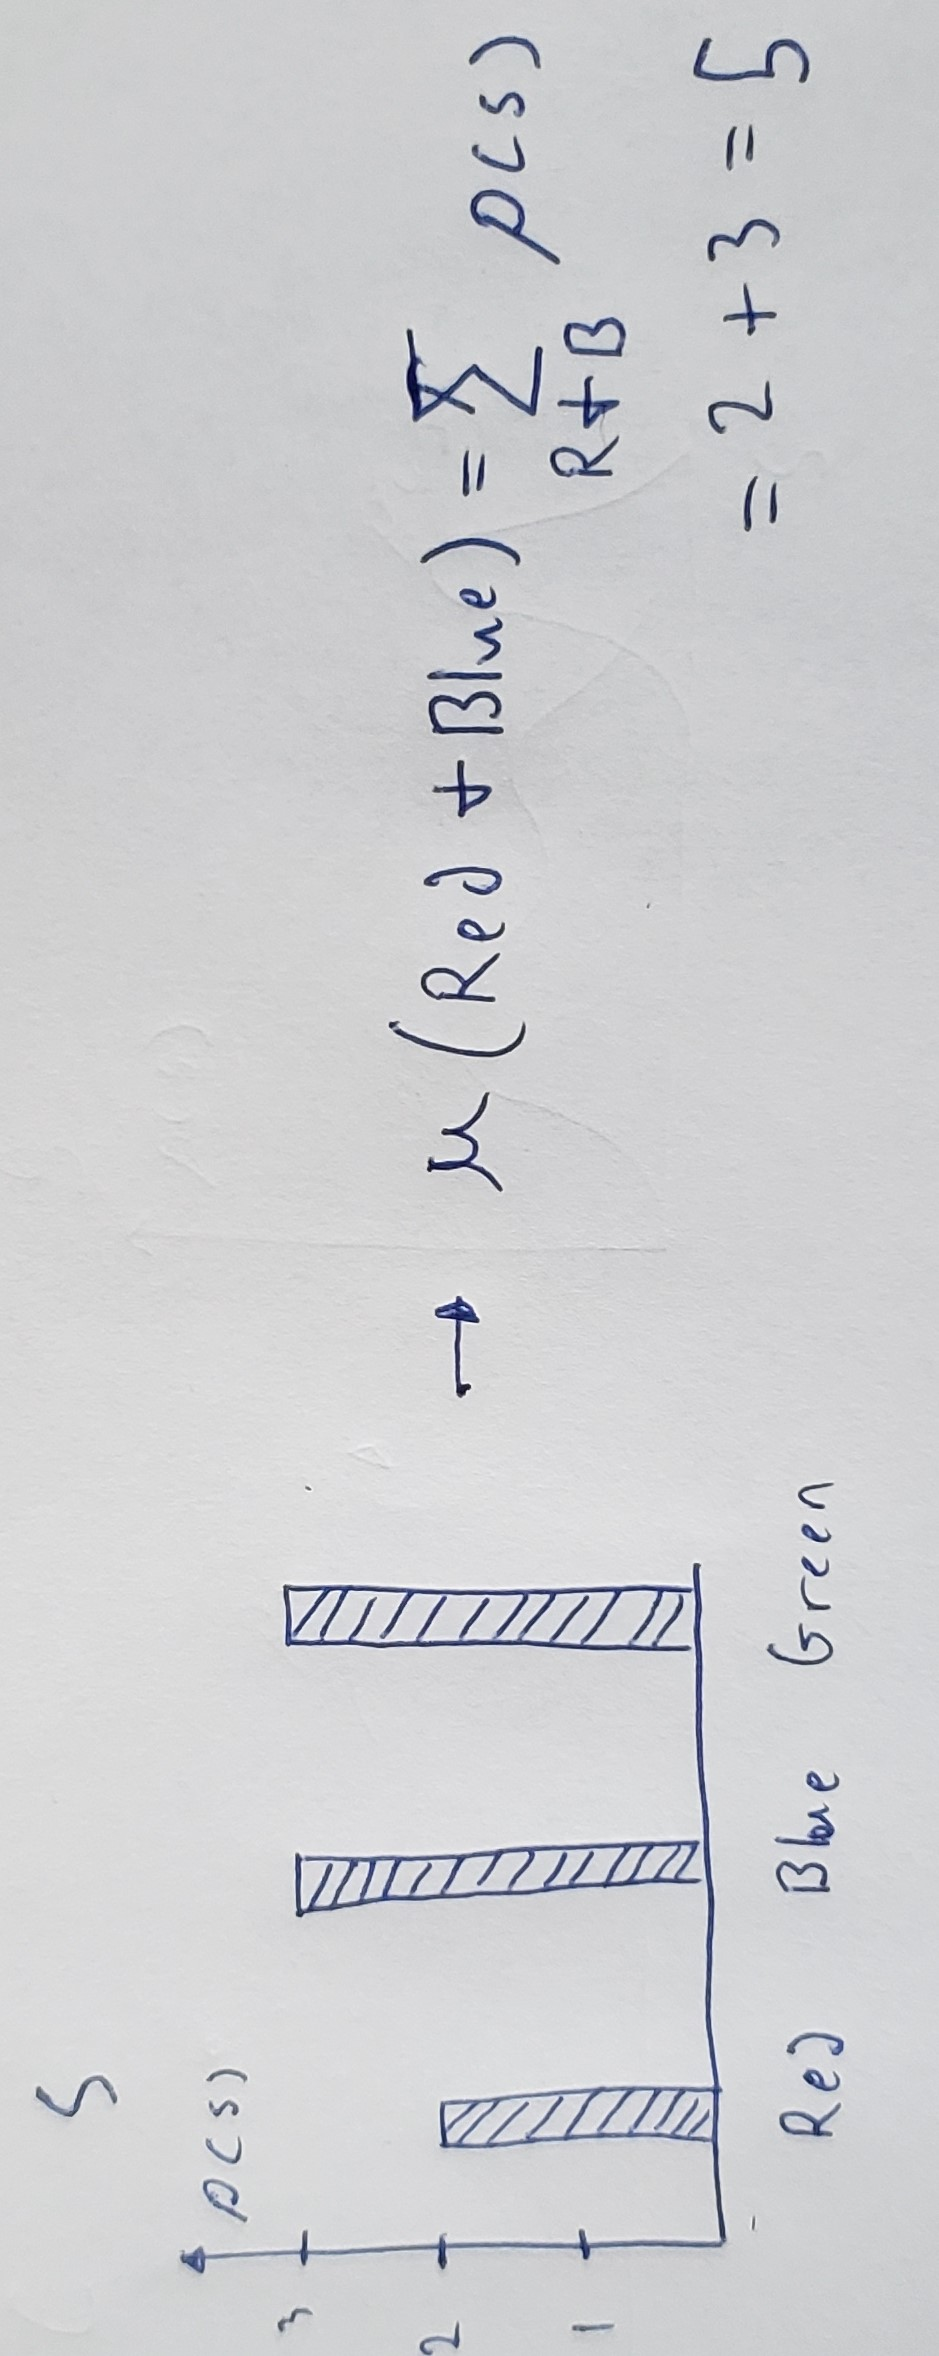
\includegraphics[width=\textwidth,angle=-90,scale=.35]{diagram3.jpg}}
\caption{Discrete example of our counting function $\mu(U)$. (not normalized)}
\end{figure}
	
	\emph{formalize continuous case}	
	
	If our system is continuous the main ideas above hold, but we must make two changes to the formalization. First, we write $\rho : \mathcal{S} \to \mathbb{R}$ as a density of states over the space and second, for $\mu$ instead of a sum we use an integral: $\mu(U) = \int_{U} \rho(s) d\mathcal{S}$ where $d\mathcal{S}$ gives the number of states in an infinitesimal area. We will continue to work in the continuous case unless otherwise stated.
	
\begin{figure}[!ht]
\centerline{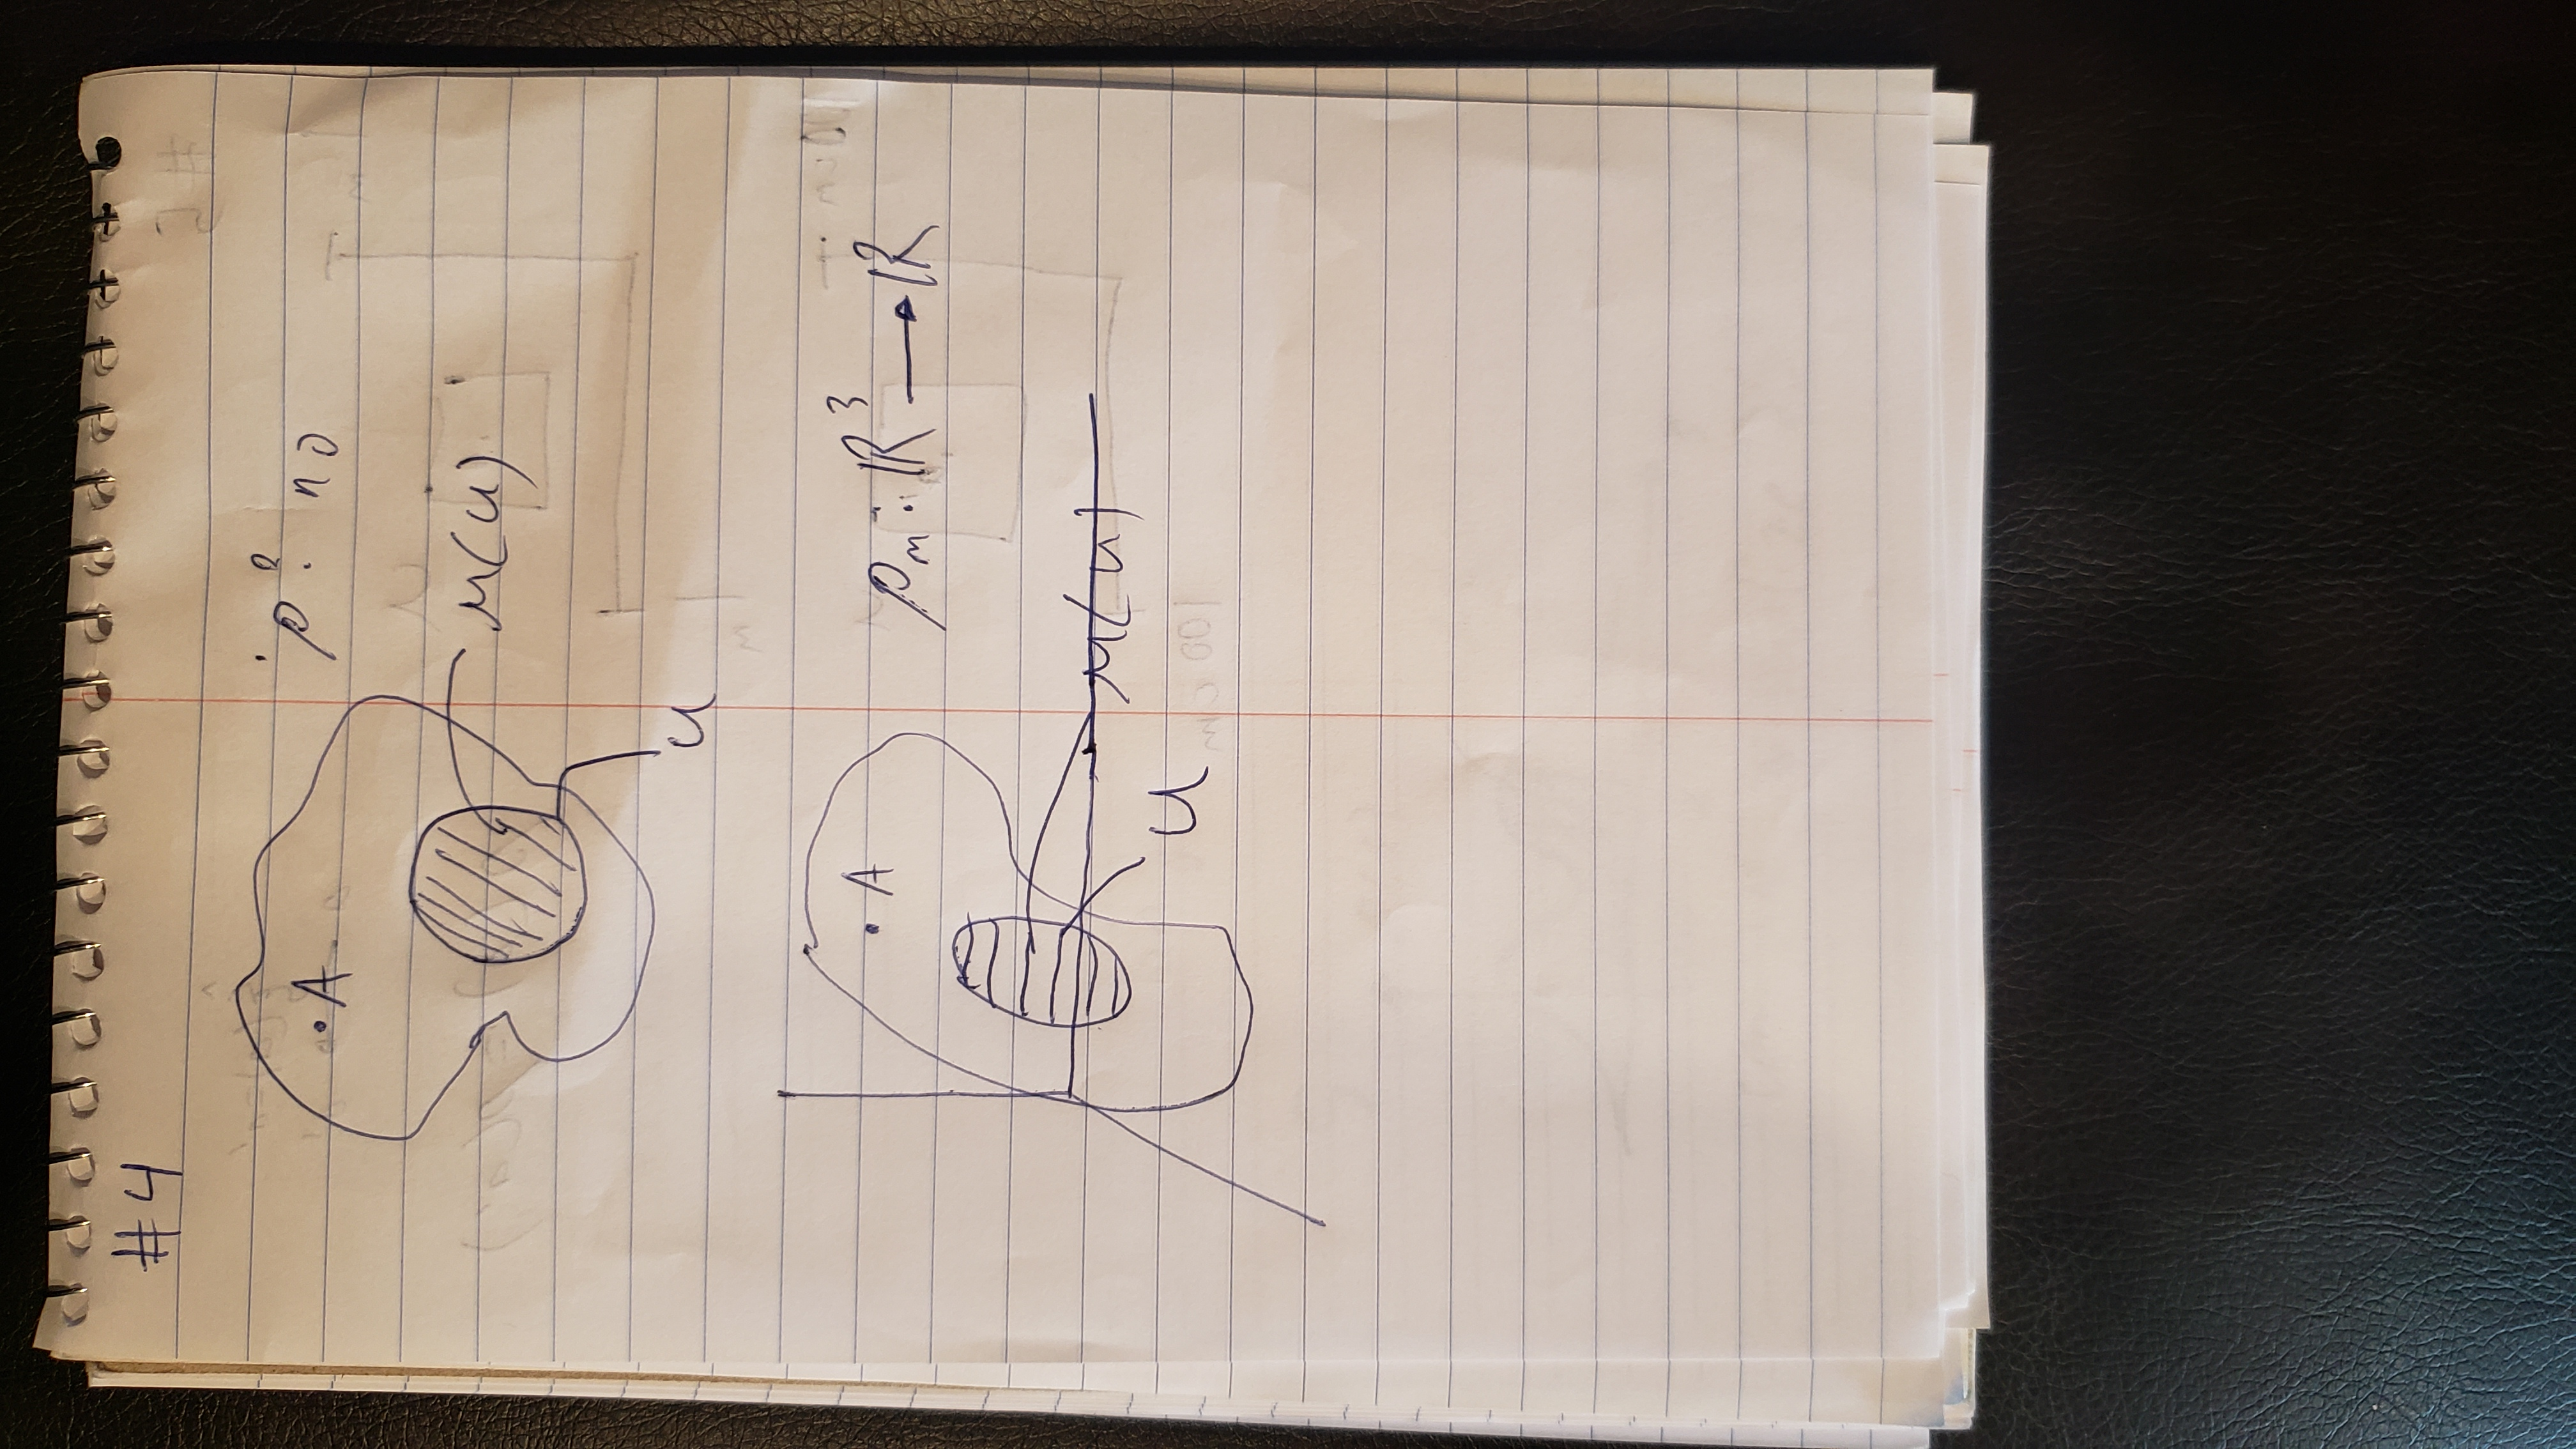
\includegraphics[width=\textwidth,angle=-90,scale=.45]{diagram4.jpg}}
\caption{Continuous example of our counting function $\mu(U)$.}
\end{figure}
	
\begin{defn}
	Let $\mathcal{C}$ be the state space of a system. The system is \textbf{infinitesimally reducible} to the infinitesimal parts (i.e. particles) identified by the state space $\mathcal{S}$ if there exists a measure $dS$ such that for every $c \in \mathcal{C}$ we can find a $\rho : \mathcal{S} \to \mathbb{R}$ such that for every $U \subseteq \mathcal{S}$ the integral $\mu(U) = \int_U \rho(s) dS$ corresponds to the fraction of the system whose parts occupy those states, which means $\mu(S) = 1$.
\end{defn}	
	
\subsection{Constraint on Coordinate Transformations}	

We can now express density in terms of state variables. These state variables must be differentiable.

Prop - the state space must be a differentiable manifold

How should the change of state variable affect the density (units/value)?

On one side, it should be invariant. rho(s), like a temperate

On the other hand, units of the density are affected by the units of the state variables (mass example, include cart -> polar)

How do we solve this? Restrict state variable to "canonical", those that allow us to express the density in the correct units.

Jacobian must be unitary under canonical transformation

Prop - the state space must allow state variables that allow the expression of the density in the correct units (canoncial). Canonical transformations must have unitary and dimensionless Jacobian.


	\emph{motivate necessity of labeling state space with numbers}	
	
	We know that for a continuous state space $\rho$ should be a density. This requires some mathematical considerations. Let's consider a typical example of a density: mass distributed over three dimensional space $\mathcal{M}$. We can talk about points in this space in a coordinate independent way.\footnote{Throughout this work we will use "coordinate" and "state variable" interchangeably. Coordinates usually denote some kind of spatial unit while state variables could represent any quantity, but in state space these are functionally the same.} Take a point $A \in \mathcal{M}$; this is the same point in all references, and we do not need to have a coordinate system defined to talk about point $A$. Now, if I have a mass distribution, and I ask you how much mass is there in a region $U \subseteq \mathcal{M}$, this is also coordinate independent as the definition of $U$ does not require a coordinate system. If I ask for the mass density at a point, however, I need to specify a quantity like $kg/m^3$. Formally, I have to specify a \textit{unit system} of the space. In math terms this means that $\rho_m : \mathbb{R}^3 \to \mathbb{R}$ not $\rho_m : \mathcal{M} \to \mathbb{R}$. We cannot define a map directly from $\mathcal{M}$ to $\mathbb{R}$. If we were to change our unit system to $g/km^3$ the actual numerical value of the density at each point changes; the density varies with the choice of coordinates.\footnote{Here we used "coordinate" and "unit" interchangeably. We will see later what the exact definition of a unit is, but for now they can be thought of as equivalent.}
	
%\begin{figure}[!ht]
%\centerline{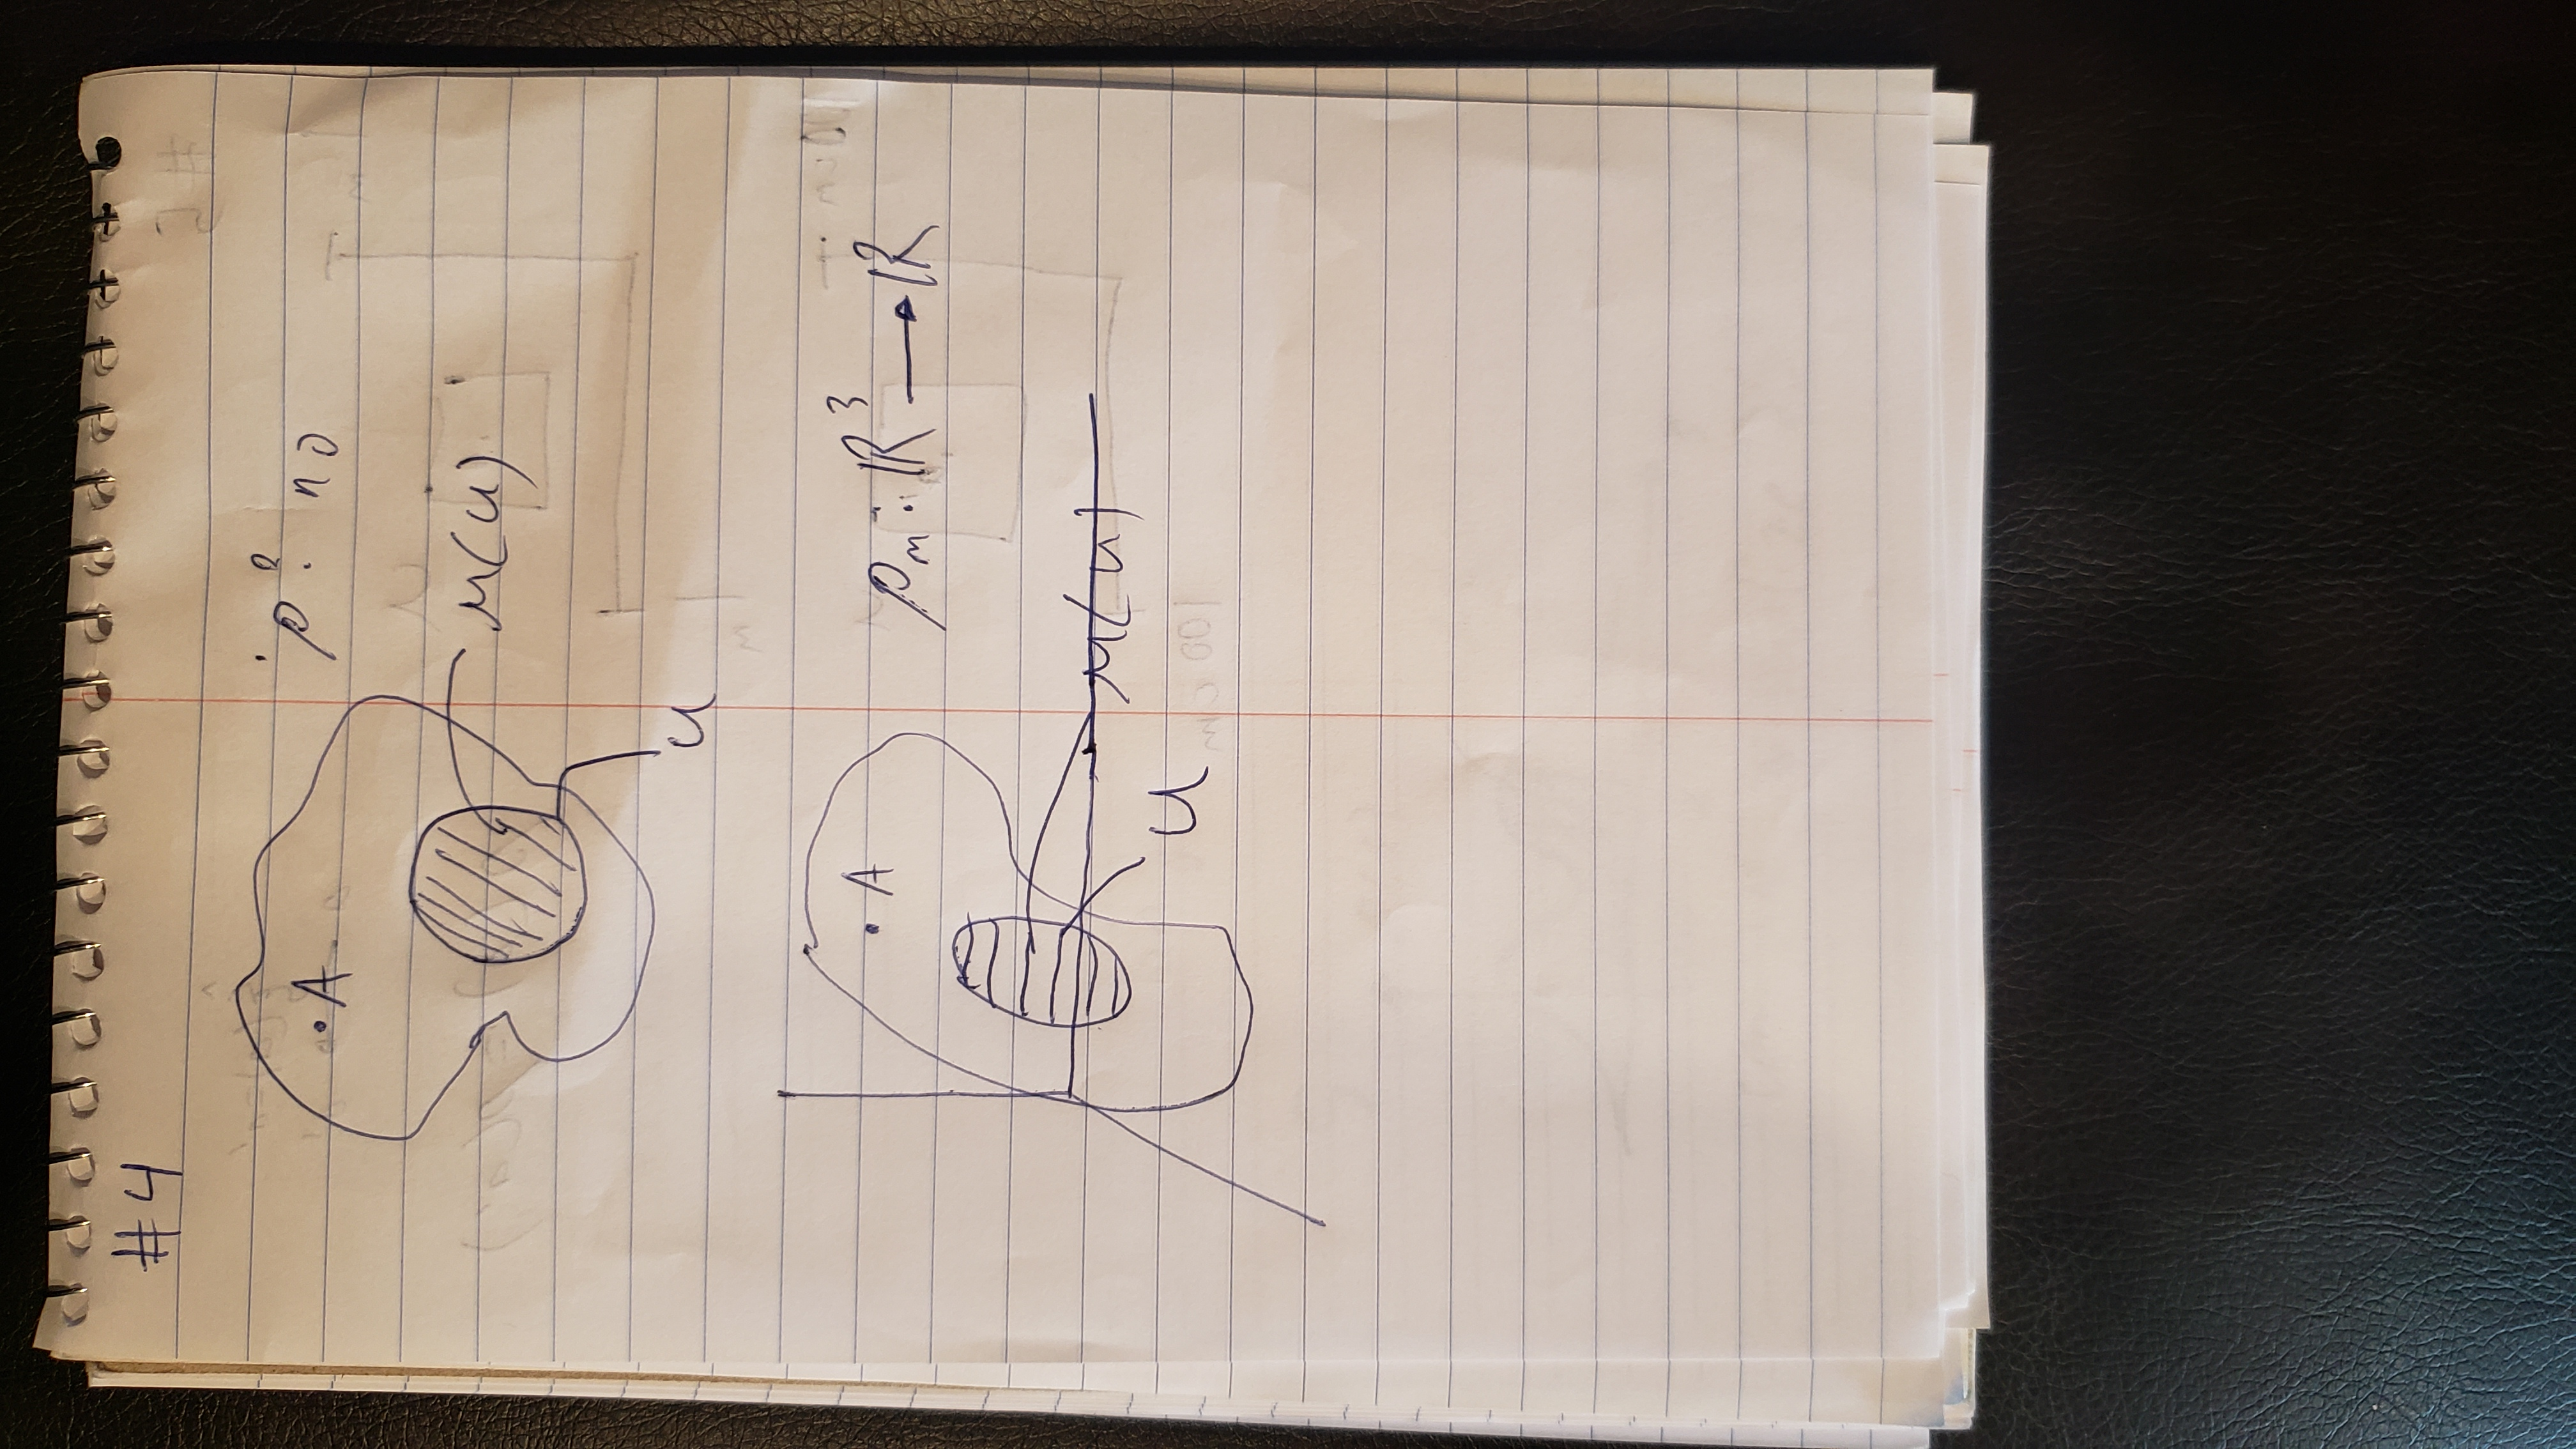
\includegraphics[width=\textwidth,angle=-90,scale=.45]{diagram4.jpg}}
%\caption{Without defining a measure we cannot define our density.}
%\end{figure}
	
	We have seen that to define a density we must define a way of labeling our space numerically so that we have something that looks like a volume element. If we want to further describe the state of the system we need to identify our states in $\mathcal{S}$ with numbers so that all states are uniquely labeled. This system of labeling will give us our \textit{state variables} or coordinates. 

\begin{defn}
	A state variable assigns one numerical quantity to each state. Formally, it is a map $\xi : \mathcal{S} \to \mathbb{R}$. A complete set of state variables fully identifies a state. Formally, it is an invertible  map $\xi^a : S \rightarrow \mathbb{R}^n $.
\end{defn}

\emph{Discussion on units. Write $\rho$ as a density. Clarify density vs distribution} 
	
	Because we want $\rho$ to be a density we must write it in terms of our state variables $\xi^a$ i.e. we write $\rho$ as a map $\rho_\xi: \mathbb{R}^n \to \mathbb{R}$. We know $\xi^a$ is an invertible map between $\mathbb{R}^n$ and our state space $\mathcal{S}$ so we can write its inverse as $\xi^{-1} : \mathbb{R}^n \to \mathcal{S}$. Taking this we can write $\rho_c(s)$ with $s = \xi^{-1}(\xi^a)$ to get $\rho_\xi$. This will give us a density of states over our state space. Note that the density and the distribution are distinct quantities; specifically the distribution is $\rho_c : \mathcal{S} \to \mathbb{R}$ and the density is $\rho_{\xi} : \mathbb{R}^n \to \mathbb{R}$. The density requires labeling the space with coordinates to be defined while the distribution does not.\emph{why do we refer mostly to the density?}\footnote{Note that we will use $\xi^a, \xi^b, \xi^c$ for state variables; $q^i, q^j, q^k$ for unit variables; $\xi^\alpha, \xi^\beta, \xi^\gamma$ for state variables that include time (i.e. four momentum). For distributions/densities we use $\rho$; where we need to distinguish between the two we will use $\rho_c$ for the distribution and $\rho_\xi$ for the density. States are indicated with $s$ and state variables with $\xi$. Also note the duplicity of $\rho$, $s$, and $\xi$. We use $\rho(s)$ as $\mathcal{S} \to \mathbb{R}$; $\rho(\xi^a)$ as $\mathbb{R}^n \to \mathbb{R}$; $\rho(\hat{\xi}^b)$ as $\mathbb{R}^n \to \mathbb{R}$; $\xi^a(s)$ as $\mathcal{S} \to \mathbb{R}^n$; $s(\xi^a)$ as $\mathbb{R}^n \to \mathcal{S}$.
Thus we have the following identities: $\rho(s(\xi^a)) = \rho(\xi^a)$; $\rho(s) = \rho(s (\xi^a(s)))$.}

\emph{give example of coordinate independent quantity to get reader to think about what that means; clarify independent/dependent vs invariant}

	We have seen that densities requires a defined coordinate system and that they can vary with the choice of those coordinates. What is a quantity that doesn't require a coordinate system to be well defined? One example is temperature. We can give the temperature at a point in space without a coordinate system; it is coordinate independent. There is no need for a conception any other unit to define the temperature. Formally this means we can write $T : \mathcal{M} \to \mathbb{R}$; this is a direct map from space-time to a number, we do not need to label space-time using a coordinate system. This independence also means logically that changing our coordinate system does not change the numerical value of temperature at a point. So temperature is invariant under change of coordinates.\footnote{We say coordinate independent to mean can be defined without a specified coordinate system; to be coordinate invariant means there will be no change under a change of variables. Some coordinate dependent quantities are coordinate invariant, but coordinate independent quantities are always coordinate invariant.} What exact properties does our density of states, $\rho$ exhibit?

	\emph{show that $\rho$ is coordinate invariant}
	
	We cannot discuss the value of $\rho$ without specifying a coordinate system. Without a sense of area or volume, we cannot specify a density. Thus our density is coordinate dependent. How does a change of coordinates affect it? We know that the counting function $\mu(U)$ is conserved. The number of classical particles in a region of state space does not change when we change the coordinates labeling that space. We have to account for this. Our density $\rho$ must not change when we change coordinates because the integral $\int_U \rho(s) d\mathcal{S}$ must be constant; $\rho$ cannot change under a change of variables because the number of particles in a region of state space does not change. So $\rho$ must be coordinate invariant.
	
	\emph{justify transforming as a density, differentiable change of variables}

	We can write our $\mu(U)$ as $\mu(U) = \int_{\xi(U)} \rho(\xi^a)d\xi^a$. If we change our state variables we know that that fraction of the system in a region $U \subset \mathcal{S}$ will not change. Let $\hat{\xi}^b = \hat{\xi}^b(\xi^a)$ be our change of variables. This gives us $\mu(U) = \int_{\xi(U)} \rho(\xi^a)d\xi^a = \int_{\hat{\xi}(U)} \rho(\hat{\xi}^b)d\hat{\xi}^b$. Using our transformation rule we can write $\int_{\hat{\xi}(U)} \rho(\hat{\xi}^b)d\hat{\xi}^b = \int_{\xi(U)} \rho(\hat{\xi}^b)\left|\frac{\partial\hat{\xi}^b}{\partial\xi^a}\right|d\xi^a = \int_{\xi(U)} \rho(\xi^a)d\xi^a$ where $\left|\frac{\partial\hat{\xi}^b}{\partial\xi^a}\right|$ is the Jacobian of this change of state variables. \emph{justification of changing like density} We also know that this change of variables must be differentiable otherwise the Jacobian will not be well defined.
	
Diagram 4 here 

\begin{prop}
	Because it is a density and is coordinate invariant, $\rho$ will transform as a scalar and a density under a differentiable change of state variables $\hat{\xi}^b = \hat{\xi}^b(\xi^a)$.
\end{prop}

	\emph{combine everything above to get unitary jacobian requirement}

	Armed with this knowledge we can derive our mathematical constraints on changes of state variables. We already know $\rho(\xi^a) = \rho(\hat{\xi}^b)$ by proposition 3; we can drop the integral from $\int_{\xi(U)} \rho(\hat{\xi}^b)\left|\frac{\partial\hat{\xi}^b}{\partial\xi^a}\right|d\xi^a = \int_{\xi(U)} \rho(\xi^a)d\xi^a$ to get $\rho(\xi^a) = \rho(\hat{\xi}^b)\left|\frac{\partial\hat{\xi}^b}{\partial\xi^a}\right|$ which implies that $\left|\frac{\partial\hat{\xi}^b}{\partial\xi^a}\right| = 1$ and is dimensionless.\emph{where should we make the point that the units of $\rho$ don't change?}
		
\begin{prop}
	A change of state variables must be differentiable and must have a unitary Jacobian i.e. $\left|\frac{\partial\hat{\xi}^b}{\partial\xi^a}\right| = 1$.
\end{prop}

\emph{corollary conservation of areas/volumes? with diagram}

\subsection{Unit Variables, Conjugate Pairs, and 2n Dimensional State Space}

\emph{Talk about unit system in general: some choices are free, some are dependent. Give example of dependent/independent unit variables (like velocity down). Example needs refining.}

	We will now defined a unit system using a select number of our state variables which we will call unit variables. If we change one of these unit variables, we will also have to change any other state variables that depend on the definition of the unit we changed. For example if $q^1$ defines the position relative to the x-axis in meters and $k_1$ is the velocity relative to the x-axis in meters per second, a change in $q^1$ to kilometers would necessitate a change in $k_1$ to kilometers per second. So a change of units $\hat{q}^j = \hat{q}^j(q^i)$ will induce a unique change of state variables $\hat{\xi}^b = \hat{\xi}^b(\xi^a)$. Some choices of unit variables are independent of each other i.e. charge and mass, but many are not i.e. distance and velocity along the same axis. \emph{improve this example}

\begin{defn}
	We define a unit variable $q \in \xi^a$ as a state variable that is the definition of a unit. The set of unit variables $q^i \in \xi^a$ defines a unit system upon which the other state variables depend.
\end{defn}

	Now we want to understand what happens under a change of unit variables. What is the correct corresponding change of state variables that corresponds with a change in unit variables? 
	
	Let's start with the simplest case: one variables suffices to describe our unit system. We then can write our set of state variables as $\xi^a = \{q,k^a\}$ where $k^a$ could represent any number of state variables. Let's suppose we performed a change of units. We then have $\hat{q}^j = \hat{q}^j(q^i)$. What are the restrictions on the set of $k^a$'s? We can use the fact that the Jacobian of any change of state variables must be unitary to show that there exists exactly one $k^a$. 
	
	Now we allow and arbitrary number of $q^i$'s to define our unit system. Using the same process as above we show that for each $q^i$ there must be exactly one $k^a$. This means that our state space $\mathcal{S}$ must be $2n$ dimensional and that our state variables come in pairs consisting of one unit variable and one dependent state variable. (The typical course in mechanics defines Hamiltonian Mechanics in terms of position-momentum pairs).\footnote{For a full, mathematically rigorous derivation see: PLACEHOLDER}

\begin{prop}
	The state space of the particles is $2n$ dimensional. The state variables are organized in pairs $\{q^i, k_i\}$ where the set $\{q^i\}$ defines the unit system. These state variables have a well defined transformation rule with a unitary Jacobian.
\end{prop}

\subsection{Degrees of Freedom, Areas in State Space, and Poisson Brackets}

\begin{defn}
	A degree of freedom is a pair $\{q^i,k_i\}$. Degrees of freedom are orthogonal 2D surfaces in phase space.
\end{defn}
	
\begin{prop}
	For each independent degree of freedom, the area given $\int_U \hbar dq^i dk_i = \int_U dq^i dp_i$ quantifies the number of possible configurations within the region $U$.
\end{prop}

\begin{defn}
	The Poisson bracket is defined as $\{f,g\} = \frac{\partial f}{\partial x}\frac{\partial g}{\partial p} - \frac{\partial g}{\partial x}\frac{\partial f}{\partial p}$.
\end{defn}

\begin{prop}
	The Poisson bracket $\{f, g\}$ translates the densities of states into densities per unit area of $f, g$. It is the Jacobian of the transformation $dfdg \rightarrow dxdp$ i.e. $dfdg = \{f,g\}dxdp$.
\end{prop}
	
\section{Reversible and Deterministic Evolution}

\begin{assump}[Reversible and Deterministic Evolution]
	The system undergoes Reversible and Deterministic Evolution meaning given the state of the system at any time, its state at all past and future times is known.
\end{assump}

Particle states change in time. But we have a law of how to go from one state to the other. Bijection $\mathcal{T}_{\Delta t} : \mathcal{S} \to \mathcal{S}$ ... This only gives you the infinitesimal displacement in time.

\begin{defn}
	We write $\lambda: \mathbb{R} \rightarrow \mathcal{S}$ defined as $s = \lambda(t)$ as the evolution of the state of one particle. Now the density associated with the state at $t_0$ is given by $\rho_c(\lambda(t_0),t_0)$.
\end{defn}

	%By our condition of Deterministic and Reversible evolution we must have $\rho(\lambda(t_0),t_0) = \rho(\lambda(t),t)$ meaning this density of states is conserved over time. So all particles that begin in the same state will evolve through and end in the same states. Now going back to our integral $\int_{\Sigma} \rho_c\omega(d\Sigma)$ we will find that our region $\Sigma$ is mapped to a new region in state space as the system evolves, but the same fraction of the parts of the system will be found in that region.
	
As particle states move, the will "drag" along the same evolution all the particles that are associated with that state. This is going to tell you that the infinitesimal displacement is "divergenceless" (conserves density)

\begin{prop}
	The density $\rho_c(s,t)$ in conserved. This means that while particles may change state over the course of the system's evolution, any particles that begin in the same state will be found in the same state throughout the evolution no matter what point in time is chosen. So we have $\rho(\lambda(t_0),t_0) = \rho(\lambda(t),t)$. (diagram showing conserved volumes/areas)
\end{prop}

\begin{prop}
	The above conditions are sufficient to say that our system is Hamiltonian and thus satisfies Hamilton's equations. So the evolution of the system can be written in the familiar way:
	$$d_tq^i = \partial_{p_i}H$$
	$$d_tp_i = -\partial_{q^i}H$$
\end{prop} 
	
	%The incredible thing here is that from two assumptions we can derive the entirety of Hamiltonian mechanics. 

\section{Kinematic Equivalence}

\begin{assump}[Kinematic Equivalence]
	(More physicsy) Trajectories in space-time suffice to recover trajectories in phase space. We know the precise trajectory in phase space given a trajectory in physical space-time; there is an invertible bijection between the two.(diagram showing bijection)
\end{assump}

\subsection{Weak Equivalence}

\begin{defn}
	We take $x^i = q^i$. We then define $v_i = d_tx^i$. Weak equivalence means $v_i(q^i, p_i)$ is invertible.
\end{defn}

(photon counter-example $v^i$ function only of $x^i$)

\begin{prop}
	A classical system that satisfies weak equivalence is a Lagrangian system. Formally, we can a define a Lagrangian $\mathcal{L}$ that is convex and has unique solutions.
\end{prop}

\subsection{Full Equivalence}

The units that are used to express the density on position and velocity must be dependent only on $q^i$ if they are to fully define the unit system.

\begin{defn}
	Full equivalence means that Kinematic Equivalence extends to the composite system. So we have $\rho(q^i,p_j) = \left|J\right|\rho(x^i,v^j) = \left|\frac{\partial v^i}{\partial p_j}\right|\rho(x^i,v^j)$. The Jacobian is only a function of $q^i$.
\end{defn}

\begin{prop}
	A system that satisfies full kinematic equivalence obeys the laws of massive particles under potential forces.
\end{prop}

\section{Advanced topics}

\subsection{Action Principle}

The action principle that many courses in mechanics take \emph{a priori} is simple a consequence of our assumptions. We can find a physical justification for our mathematical structures.

\subsection{Kinematic vs dynamics}

Differences between Newtonian/Lagrangian/Hamiltonian mechanics.

Show that they are inequivalent. Newtonian mechanics needs n functions to define the evolution while Lagrangian/Hamiltonian requires 1. All Lagrangians that have unique solution have a Hamiltonian. All Hamiltonians have unique solutions, but not necessarily a Lagrangian. (must follow discussion on the action principle) Mix with examples.

Kinematics and dynamics. Newtonian and Hamiltonian mechanics necessarily define both. Technically, Lagrangian mechanics is purely kinematic (equations are only in terms of position and velocity - you can't distinguish apparent forces from real forces). The only way to recover the dynamics is to assume the system is also Hamiltonian.

Kinematic aliasing (systems with different dynamics may have the same kinematics). Example of 3 different dynamics (friction, boosted, losing mass). This is confusing because, in some cases, you can treat non-conservative systems in Lagrangian mechanics as they look like conservative systems in a non-inertial frame (naturally, the Hamiltonian and the conjugate momentum will not correspond to what you expect).

How is kinematic aliasing resolved. Newtonian mechanics resolves kinematic aliasing by invoking inertial frames and by writing equations that are valid \emph{only} in inertial frames (you can distinguish apparent forces from real forces in an inertial frame).  In Lagrangian/Hamiltonian mechanics, the equations are invariant under coordinate transformation: we can't do that anymore. You fix the system to be conservative. If you had a system of equations that were invariant under all coordinate transformation for all frames, you would not be able to tell which forces are apparent and which forces are real.

\subsection{Entropy in classical mechanics}

Entropy is invariant under coordinate transformation - the same for all observers (invariance under time is less important).

Classical uncertainty principle: fixing the entropy of the distribution gives us an inequality that is saturated by Gaussian distributions. (discuss parallel with quantum mechanics - classical mechanics allow for minus infinite entropy)

Time evolution of entropy. It is conserved only under Hamiltonian evolution. If the evolution is not Hamiltonian, the entropy does the opposite of what one expected. (dissipative systems, like damped harmonic oscillator, concentrate the distributions around the attractor, and therefore) The problem is that the same statement at different time provides different amount of information/granularity of the description.


\section{Conclusion}
	
















\end{document}
